\begin{XeClass}{FsUrlConnection}
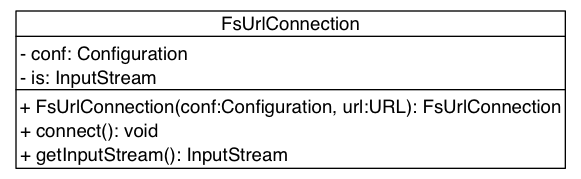
\includegraphics[width=10cm]{cdig/FsUrlConnection.png}
     
 URL连接到InputStreams上的类
 具有Configuration对象conf和InputStream对象is作为实例属性
 继承自URLConnection的connect方法和getInputStream方法,并Override覆盖其原来方法
 构造函数接收两个参数,第一个参数是Configuration conf.
 第二个参数是URL对象url,调用其超类URLConnection构造函数super(url)

    \begin{XeMethod}{\XePublic}{void}{connect}
         
 connect方法是继承自URLConnection,在FsUrlConnection类中Override的方法
 该方法通过FileSystem.get(url.toURI(), conf)方法获得FileSystem对象fs
 并用fs打开url的地址获得的输入流对象赋值给FsUrlConnection类的实例变量is

    \end{XeMethod}

    \begin{XeMethod}{\XePublic}{InputStream}{getInputStream}
         
 getInputStream()方法是继承自URLConnection,在FsUrlConnection类中Override的方法
 该方法首先判断FsUrlConnection类的实例变量is是否为null,若为null则调用connect方法

    \end{XeMethod}

\end{XeClass}
